\documentclass[11pt,a4paper,oneside]{report}

\usepackage{amsmath}
\usepackage{graphicx}

\graphicspath{ {./images/} }

\begin{document}
\section{Stator equations in ABC Coordinates}

\begin{center}
	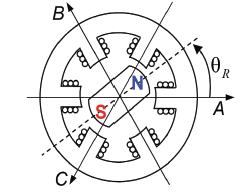
\includegraphics[scale=1]{bldc}
\end{center}

Stator equations in the case of star-connection in ABC coordinates

\begin{equation}
	\left\{
	\begin{split}
		U_{af} = \frac{d\psi_a}{dt}+I_aR_f\\
		U_{bf} = \frac{d\psi_b}{dt}+I_bR_f\\
		U_{cf} = \frac{d\psi_c}{dt}+I_cR_f\\
	\end{split}
	\right.
\end{equation}
where $U_{a,b,c}$ are phase voltages, $\psi_{a,b,c}$ are phase flux linkages, $I_{a,b,c}$ are phase currents, $R_f$ is a phase resistance.

Fluxes in armatures are induced by self current, magnetic fields of other phases and magnetic field of rotor:

 \begin{equation}
 	\left\{
 	\begin{split}
 		\psi_a = L_aI_a+L_{ab}I_b+L_{ac}I_c+\phi_{fa}\\
 		\psi_b = L_bI_b+L_{ab}I_b+L_{bc}I_c+\phi_{fb}\\
 		\psi_c = L_cI_c+L_{ac}I_c+L_{bc}I_b+\phi_{fc}
 	\end{split}
 	\right.
 \end{equation}
where $L_{a,b,c}$ are phase armatures inductance, $L_{ab,bc,ac}$ re two phase cross-inductance, $\psi_{fa,fb,fc}$ are flux linkages induced by rotor.

For non-salinet motors (cylindrical rotor) inductance and cross-inductance don't depend on rotor angle. For this case denote $L_f$ phase armature inductance, $L_{ff}$ cross-inductances. Therefore
\begin{equation}
\left\{
\begin{split}
	U_{af} = L_f\frac{dI_a}{dt}+L_{ff}\frac{dI_b}{dt}+L_{ff}\frac{dI_c}{dt}+\frac{d\psi_a}{dt}+I_aR\\
	U_{bf} = L_f\frac{dI_b}{dt}+L_{ff}\frac{dI_a}{dt}+L_{ff}\frac{dI_c}{dt}+\frac{d\psi_b}{dt}+I_bR\\
	U_{cf} = L_f\frac{dI_c}{dt}+L_{ff}\frac{dI_a}{dt}+L_{ff}\frac{dI_b}{dt}+\frac{d\psi_c}{dt}+I_cR\\
\end{split}
\right.
\end{equation}

It should be noted that $\frac{d\psi_{a,b,c}}{dt}$ are EMF induced in stator armatures by rotor.
\begin{equation}
	\label{phase-volt_eq}
	\left\{
\begin{split}
	U_{af} = L_f\frac{dI_a}{dt}+L_{ff}\frac{dI_b}{dt}+L_{ff}\frac{dI_c}{dt}E_a+I_aR\\
	U_{bf} = L_f\frac{dI_b}{dt}+L_{ff}\frac{dI_a}{dt}+L_{ff}\frac{dI_c}{dt}+E_b+I_bR\\
	U_{cf} = L_f\frac{dI_c}{dt}+L_{ff}\frac{dI_a}{dt}+L_{ff}\frac{dI_b}{dt}+E_c+I_cR\\
\end{split}
\right.
\end{equation}

Replace phase voltages by linear voltages (respectively with zero point in the case of star connection):

\begin{equation}
	\label{phase-linear}
	\left\{
	\begin{split}
		U_a-U_b=U_{af}-U_{bf}\\
		U_b-U_c=U_{bf}-U_{cf}\\
		U_c-U_a=U_{cf}-U_{af}\\
	\end{split}
	\right.
\end{equation}

Combining (\ref{phase-volt_eq}) and (\ref{phase-linear}) yields

\begin{equation}
	\label{phase-linear}
	\left\{
	\begin{split}
		\frac{d}{dt}I_a=\frac{1}{L_f-L_{ff}}\left(U_a-U_b+(L_f-L_{ff})\frac{d}{dt}I_b-E_a+E_b-R(I_a-I_b) \right)\\
		\frac{d}{dt}I_b=\frac{1}{L_f-L_{ff}}\left(U_b-U_c+(L_f-L_{ff})\frac{d}{dt}I_c-E_b+E_c-R(I_b-I_c) \right)\\
		\frac{d}{dt}I_c=\frac{1}{L_f-L_{ff}}\left(U_c-U_a+(L_f-L_{ff})\frac{d}{dt}I_a-E_c+E_a-R(I_c-I_a) \right)\\
	\end{split}
	\right.
\end{equation}

Introduce unity EMF function that depends on rotor angle

\begin{center}
	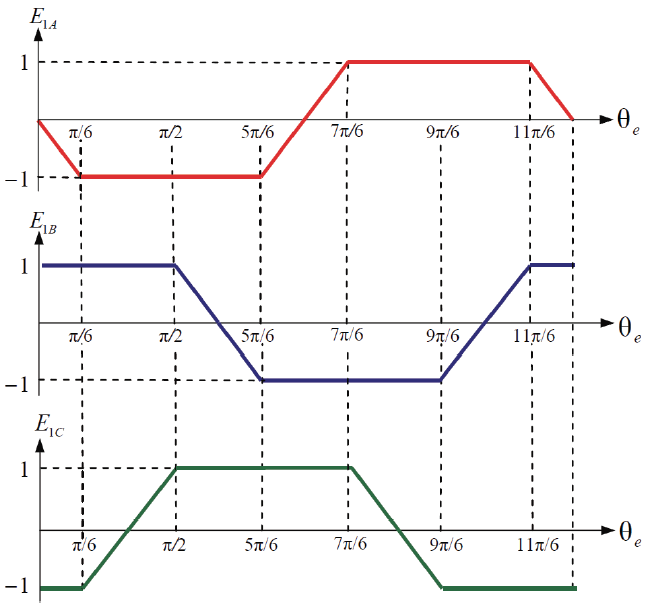
\includegraphics[scale=0.7]{emf}
\end{center}

EMF values can be represented as
\begin{equation}
	\left\{
	\begin{split}
		E_a=\psi_f\omega_eE_{1a}=\psi_fZ\omega_rE_{1a}\\
		E_b=\psi_f\omega_eE_{1b}=\psi_fZ\omega_rE_{1b}\\
		E_c=\psi_f\omega_eE_{1c}=\psi_fZ\omega_rE_{1c}\\
	\end{split}
	\right.
\end{equation}
where $\psi_f$ is an flux linkage magnitude of rotor and phase armature, $\omega_e$ is an electric field velocity. $\omega_r$ is a rotor velocity, $Z$ is a number of poles pairs.

Rewrite (\ref{phase-volt_eq}) taking into account EMF equations and currents symmetry
\begin{equation}
	\left\{
	\begin{split}
		&\frac{d}{dt}I_a=\frac{d}{t}I_b+  \frac{1}{L_f-L_{ff}}\left(U_a-U_b-\psi_fZ\omega_r(E_{1a}-E_{1b})-R(I_a-I_b) \right)\\
		&\frac{d}{dt}I_b=\frac{d}{t}I_c+  \frac{1}{L_f-L_{ff}}\left(U_b-U_c-\psi_fZ\omega_r(E_{1b}-E_{1c})-R(I_b-I_c) \right)\\
		&\frac{d}{dt}I_c=\frac{d}{t}I_a+  \frac{1}{L_f-L_{ff}}\left(U_c-U_a-\psi_fZ\omega_r(E_{1c}-E_{1a})-R(I_a-I_b) \right)\\
		&\frac{d}{dt}I_a+\frac{d}{dt}I_b+\frac{d}{dt}I_c=0
	\end{split}
	\right.
\end{equation}

or in Koshi form
\begin{equation}
	\left\{
	\begin{split}
		&\frac{d}{dt}I_a=\frac{1}{3(L_f-L_{ff})}\left(U_a-U_b+U_a-U_c+\psi_fZ\omega_r(E_{1b}+E_{1c}-2E_{1a})-3RI_a\right)\\
		&\frac{d}{dt}I_b=\frac{1}{3(L_f-L_{ff})}\left(-U_a+U_b+U_b-U_c+\psi_fZ\omega_r(E_{1c}+E_{1a}-2E_{1b})-3RI_b\right)\\
		&\frac{d}{dt}I_c=\frac{1}{3(L_f-L_{ff})}\left(-U_b+U_c+U_c-U_a+\psi_fZ\omega_r(E_{1a}+E_{1b}-2E_{1c})-3RI_c\right)\\
		&\frac{d}{dt}I_a+\frac{d}{dt}I_b+\frac{d}{dt}I_c=0
	\end{split}
\right.
\end{equation}

or with Laplace transformation

\begin{equation}
	\left\{
	\begin{split}
		&I_a=\frac{k}{Tp+1}\left(2U_a-U_b-U_c+\psi_fZ\omega_r(E_{1b}+E_{1c}-2E_{1a})\right)\\
		&I_b=\frac{k}{Tp+1}\left(2U_b-U_a-U_c+\psi_fZ\omega_r(E_{1a}+E_{1c}-2E_{1b})\right)\\
		&I_c=\frac{k}{Tp+1}\left(2U_c-U_a-U_b+\psi_fZ\omega_r(E_{1a}+E_{1b}-2E_{1c})\right)\\
		& k=\frac{1}{3R}\\
		& T=\frac{L_f-L_{ff}}{R}
	\end{split}
	\right.
\end{equation}

\section{Momentum equations}

Assume that heating and reactive power transformation losses are neglecting. In this case

\begin{equation}
	I_aE_a+I_bE_b+I_cE_c=\omega_rM
\end{equation}

Therefore

\begin{equation}
	M=\frac{I_aE_a+I_bE_b+I_cE_c}{\omega_r}
\end{equation}

Taking into account EMF equations:
\begin{equation}
	M=\psi_fZ(I_aE_{1a}+I_bE_{1b}+I_cE_{1c})
\end{equation}

\section{Position sensor}

\begin{center}
	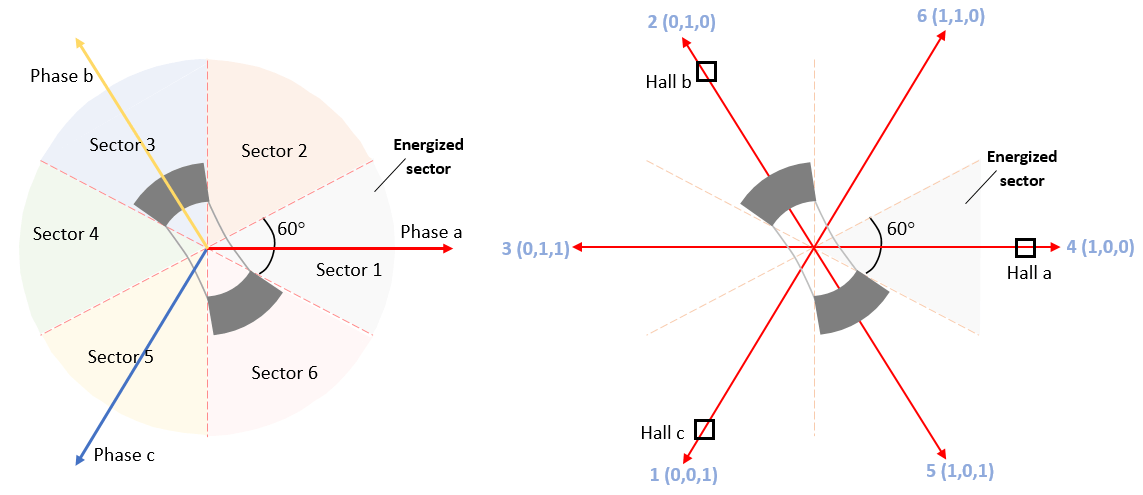
\includegraphics[scale=0.5]{sensor}
\end{center}





\end{document}